\chapter{Werken met schijven en schijfimages}

\section{Schijfstations}
\label{cha:using-disks}
\index{Schijfstations}

De MEGA65 beschikt over een ingebouwd 3.5"-diskettestation en ondersteunt externe schijfstations in Commodore-stijl via de seriële IEC-poort aan de achterzijde van de computer. De IEC-poort ondersteunt ook andere externe IEC-opslagapparaten, zoals de SD2IEC.\index{SD2IEC-apparaat} Sommige IEC-opslagapparaten kunt u in een keten aansluiten en tegelijkertijd gebruiken.

De MEGA65 bevat ook een ``virtueel'' schijfstation dat D81- of D64-schijfimagebestanden\index{D81-schijfimage}\index{D64-schijfimage} op de SD-kaart kan aankoppelen. De meeste MEGA65-programmatuur die u van het internet downloadt, heeft de vorm van een D81-schijfimage. Programma's voor de Commodore 64 worden vaak verspreid in de vorm van een D64-schijfimage. U kunt rechtstreeks vanaf de MEGA65 een nieuw D81-schijfimage aanmaken en uw BASIC-programma's op de SD-kaart opslaan, zonder dat u extra hardware nodig hebt. U kunt ook bestanden kopiëren tussen fysieke floppy-schijven en schijfimages.

Het Intro Disk-menu\index{Intro Disk} dat u zag toen u de computer voor het eerst inschakelde, is een programma op een D81-schijfimage: een bestand met de naam {\tt MEGA65.D81} op de SD-kaart. De MEGA65 is in eerste instantie geconfigureerd om dit schijfimage automatisch op te starten. U kunt dit wijzigen in het Configuratiehulpprogramma.\index{Configuratie!Hulpprogramma} (Zie ook hoofdstuk \vref{cha:configuringyourmega}.)

U kunt schijfstations en virtuele schijfimages vanuit het Freezer-menu beheren.\index{Freezer-menu} Sommige van deze handelingen kunt u uitvoeren met BASIC-commando's zoals {\bf MOUNT}.\index{BASIC 65-commando's!MOUNT}

\subsection{Unitnummers en drivenummers}
\index{Schijfstations!Unitnummers en drivenummers}
\index{Aansluitingen!IEC}

Elk schijfstation (fysiek of virtueel) wordt benaderd via een {\it unit}nummer.\index{Unitnummer (IEC-apparaten)} Bij de vintage Commodore-computers verwijst het unitnummer naar een IEC-apparaat dat op de computer is aangesloten. Commodore reserveerde de unitnummers in het bereik 0 -- 31 voor apparaten met uiteenlopende doeleinden, waarvan 8 -- 11 voor schijfstations. Hebt u ooit een Commodore 64 gebruikt en \screentext{LOAD "*",8,1} ingetypt, dan verwijst de ``8'' naar het schijfstation dat als unit 8 is aangesloten. De schijfcommando's van BASIC 65 gebruiken standaard unit 8 en aanvaarden een {\bf U}-parameter om dit te wijzigen, bijvoorbeeld: \screentext{DLOAD "MYPROGRAM",U9}\index{BASIC 65-voorbeelden!DLOAD}\index{BASIC 65-voorbeelden!LOAD}

Bij de MEGA65 kunt u een unitnummer toewijzen aan het virtuele schijfstation met een gekoppeld schijfimage, of aan het ingebouwde 3.5"-diskettestation. U moet een schijfimage of het ingebouwde 3.5"-diskettestation aan een unitnummer koppelen voordat het gebruikt kan worden. Elk bericht dat naar een unitnummer wordt gestuurd dat aan een virtuele schijf of het ingebouwde diskettestation is toegewezen, wordt door de MEGA65 afgehandeld. Alle overige berichten worden naar de seriële IEC-poort gestuurd.

Schijfcommando's aanvaarden ook een optionele parameter om een {\it drive}nummer op te geven.\index{Drivenummer (IEC-apparaten)} Deze is alleen nodig bij het aansluiten van een vintage dubbel diskettestation via de IEC-poort, zoals de Commodore 4040, 8050 of 8250. Elk schijfstation kent drivenummer 0 toe aan het eerste station. Stations met twee schijven kennen drivenummer 1 toe aan het tweede station. Dubbele schijfstations zijn gewoonlijk uitgerust met een IEEE-488-interface en hebben een IEEE-488-naar-IEC-omzetter nodig om op de MEGA65 gebruikt te kunnen worden. De schijfcommando's van BASIC 65 gebruiken standaard drive 0 en aanvaarden een {\bf D}-parameter om dit te wijzigen.


\section{Werken met virtuele schijfimages}
\index{Schijfstations!Virtuele schijfimages}

De MEGA65 biedt twee ``beheerde stations'' die de via de IEC-poort aangesloten stations aanvullen. Aan het eerste beheerde station kunt u een D81- of D64-schijfimagebestand op de SD-kaart toewijzen, of u kunt het toewijzen aan het ingebouwde 3.5"-diskettestation. Aan het tweede beheerde station kunt u eveneens een D81- of D64-schijfimagebestand toewijzen, zodat er maximaal twee virtuele schijven tegelijkertijd gekoppeld kunnen worden.\footnote{Commodore was oorspronkelijk van plan een nieuw extern 3.5"-diskettestation uit te brengen, het ``1565''-station, dat bij de Commodore 65 zou horen en op een speciale niet-IEC-poort zou worden aangesloten. Het MEGA65-project heeft de ambitie om zo'n station ooit te produceren; indien dat gebeurt, zou dit station aan het tweede beheerde station worden toegewezen.}

Het eerste beheerde station kan worden ingesteld op unit 8 of 10 en het tweede beheerde station op unit 9 of 11.

\subsection{Waar u schijfimagebestanden kunt verkrijgen}

De website MEGA65 Filehost\index{Filehost-website} herbergt een bibliotheek met MEGA65-programmatuur die door de gemeenschap is gemaakt. U kunt door de programmatuur bladeren of erin zoeken, een titel downloaden en het schijfimage vervolgens met uw pc of met het Ethernet-bestandsoverdrachtshulpprogramma naar de SD-kaart kopiëren.

\url{https://files.mega65.org/}

\subsection{Schijfimages aankoppelen met de Freezer}

Open het Freezer-menu:\index{Freezer-menu} houd \widekey{RESTORE} één seconde ingedrukt en laat de toets vervolgens los. Let op de huidige toestand van aangekoppelde stations rechtsonder op het scherm.

\begin{center}
  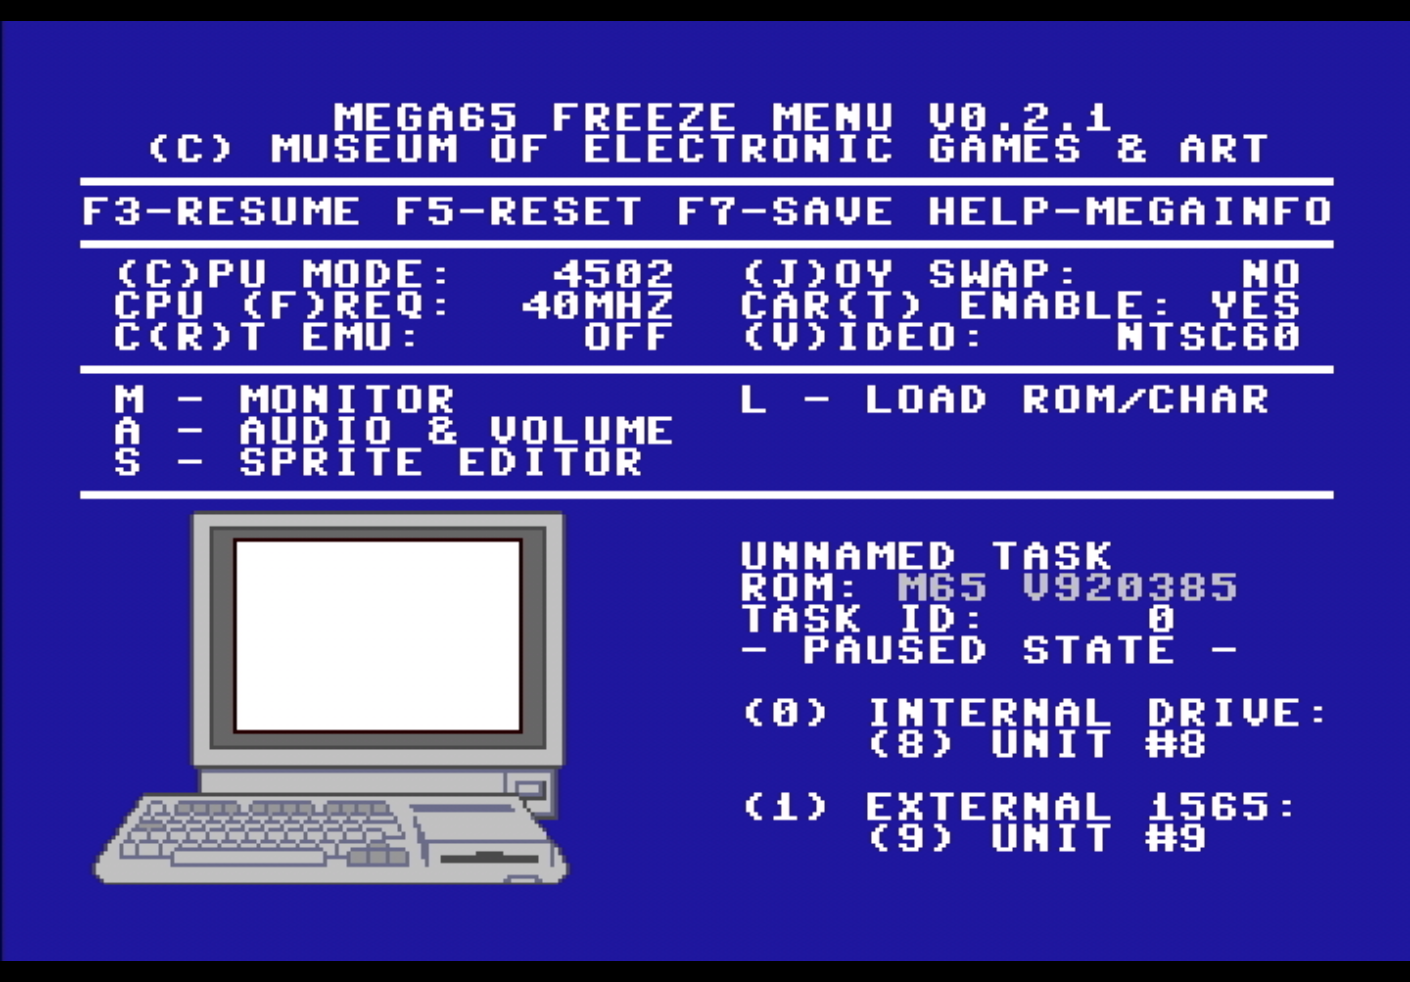
\includegraphics[width=0.7\linewidth]{images/freezer.png}
\end{center}

Om een schijfimage aan unit 8 of 10 te koppelen, selecteert u het eerste beheerde station door op \megakey{0} te drukken. Om een schijfimage aan unit 9 of 11 te koppelen, selecteert u het tweede beheerde station door op \megakey{1} te drukken. Dit opent de bestandsbrowser van de SD-kaart.

\begin{center}
  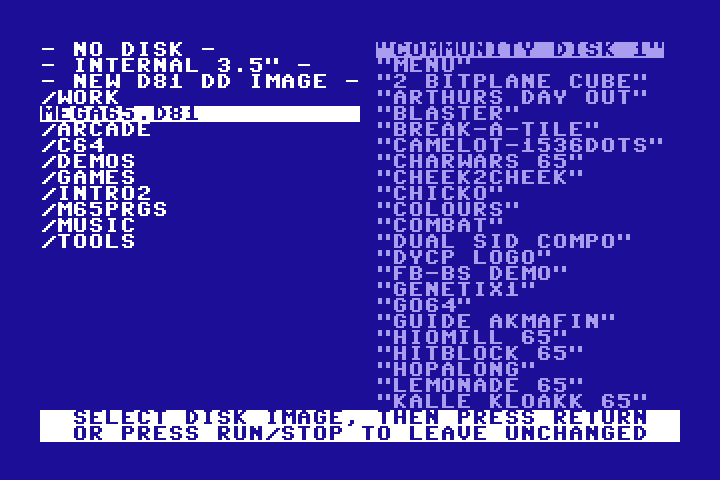
\includegraphics[width=0.7\linewidth]{images/d81-file-browser.png}
\end{center}

Gebruik de cursortoetsen om een schijfimage te selecteren en druk vervolgens op \widekey{RETURN}. Het Freezer-scherm toont dat het geselecteerde schijfimage nu aan het beheerde station is gekoppeld.

Druk vanaf het hoofdscherm van de Freezer op \megakey{8} of \megakey{9} om te wisselen tussen de unitnummers van respectievelijk het eerste en het tweede beheerde station.

\subsection{Schijfimages aankoppelen vanuit BASIC}

Met het BASIC-commando {\bf MOUNT}\index{BASIC 65-commando's!MOUNT} kunt u een schijfimage vanaf de SD-kaart aankoppelen zonder de Freezer te hoeven openen. U kunt dit commando bij de \screentext{READY}-prompt invoeren of het als onderdeel van een programma gebruiken.

Om een schijfimage aan unit 8 te koppelen, voert u {\bf MOUNT} in met de volledige bestandsnaam tussen dubbele aanhalingstekens, inclusief het achtervoegsel {\tt .D81} of {\tt .D64}:

\begin{screencode}
MOUNT "MEGA65.D81"
\end{screencode}

Om een schijfimage aan unit 9 te koppelen, geeft u het {\bf U}-argument op:

\begin{screencode}
MOUNT "MEGA65.D81",U9
\end{screencode}

\subsection{Een nieuw schijfimage aanmaken}
\index{Schijfstations!Virtuele schijfimages}

U kunt vanuit de Freezer van de MEGA65 een nieuw leeg D81-schijfimage aanmaken.\index{Freezer-menu}

\begin{enumerate}
\item Open de Freezer.\item Druk op \megakey{0} om het eerste beheerde station te selecteren.\item Selecteer boven in de bestandenlijst: \screentext{- NEW D81 DD IMAGE -}\item Voer, wanneer u daarom gevraagd wordt, een naam voor de schijf in. (Laat het achtervoegsel {\tt .D81} weg; dit wordt automatisch toegevoegd.)
\end{enumerate}

Het nieuwe schijfimage wordt op de SD-kaart aangemaakt en aan het eerste beheerde station gekoppeld. Het is geformatteerd en gereed voor gebruik.

\subsection{SD-kaartbestanden beheren in submappen}

Wanneer u enige tijd op Filehost games en toepassingen hebt gedownload, zult u uiteindelijk een grote verzameling schijfimages op uw SD-kaart hebben. Mogelijk wilt u deze bestanden in submappen ordenen. U kunt deze mappen aanmaken terwijl de SD-kaart op uw pc is aangesloten, of met het Ethernet-bestandsoverdrachtshulpprogramma.

De Freezer ondersteunt submappen in de bestandsbrowser. Elke submapnaam begint met een schuine streep (\screentext{/}). Selecteer een map om de bestanden ervan weer te geven. Om terug te keren naar de vorige map, selecteert u: \screentext{/..}

De MEGA65 houdt een ``huidige werkmap'' bij die als basismap dient voor BASIC-commando's zoals {\bf MOUNT}. Om de huidige werkmap vanuit BASIC te wijzigen, gebruikt u het {\bf CHDIR}-commando\index{BASIC 65-commando's!CHDIR} met het {\bf U12}-argument:\index{BASIC 65-voorbeelden!CHDIR}\index{BASIC 65-voorbeelden!MOUNT}

\begin{screencode}
CHDIR "DEMOS",U12

MOUNT "XANADU.D81"
\end{screencode}

\underline{OPMERKING}: De ondersteuning voor submappen op de SD-kaart is nog in ontwikkeling. Indien een schijfimage in een submap is gekoppeld, wordt het ontkoppeld door elke handeling die de huidige werkmap wijzigt. Sommige voorzieningen die bestanden gebruiken, ondersteunen mogelijk geen bestanden in submappen. Het is momenteel niet mogelijk om vanuit de Freezer een nieuw schijfimage in een submap aan te maken. Wij hopen dit in een toekomstige update te verbeteren.


\section{Het ingebouwde 3.5"-diskette\-station gebruiken}

De MEGA65 beschikt over een ingebouwd 3.5"-diskettestation, vergelijkbaar met wat voor de Commodore 65 bedoeld was. U kunt fysieke floppy-schijven gebruiken om uw programma's en gegevens op te slaan. Sommige MEGA65-programmatuur kan op diskette worden aangeschaft.

Het ingebouwde 3.5"-diskettestation moet gekoppeld worden voordat het gebruikt kan worden. Het kan aan unit 8 of unit 10 worden gekoppeld, in het eerste beheerde station.

\subsection{Het ingebouwde 3.5"-station aankoppelen met de Freezer}

Open het Freezer-menu:\index{Freezer-menu} houd \widekey{RESTORE} één seconde ingedrukt en laat de toets vervolgens los. Let op de huidige instellingen voor het aankoppelen van stations rechtsonder op het scherm.

Druk op \megakey{0} en gebruik vervolgens de pijltjestoets omlaag om \screentext{- INTERNAL 3.5" -} te selecteren. Druk op \widekey{RETURN} om de selectie te bevestigen. Het Freezer-menu toont dat het interne station aan het eerste beheerde schijfstation is gekoppeld.

Het \screentext{UNIT \#} voor het eerste station kan 8 of 10 zijn. Druk op \megakey{8} om tussen deze opties te wisselen. De schijfcommando's van BASIC 65 gebruiken standaard unit 8, dus het is gebruikelijk unit 8 te gebruiken tenzij u tegelijkertijd met meerdere schijven werkt.

Het ingebouwde 3.5"-diskettestation kan alleen in het eerste beheerde station worden gekoppeld, met unitnummers 8 of 10. Het kan niet in het tweede beheerde station worden gekoppeld (unitnummers 9 of 11).

\subsection{Het ingebouwde 3.5"-station aankoppelen vanuit BASIC}

U kunt het ingebouwde 3.5"-diskettestation met het BASIC-commando {\bf MOUNT} aan unit 8 koppelen. Dit commando werkt zowel vanaf de \screentext{READY}-prompt als vanuit een programma. Om het interne station aan unit 8 te koppelen, voert u het commando zonder argumenten in:\index{BASIC 65-voorbeelden!MOUNT}

\begin{screencode}
MOUNT
\end{screencode}

Het {\bf MOUNT}-commando kan het interne station alleen aan unit 8 koppelen. Vanuit het Freezer-menu kunt u het alleen aan unit 10 koppelen.

\subsection{DD- en HD-schijven}
\index{Schijfstations!Double-densityschijven (DD)}
\index{Schijfstations!High-densityschijven (HD)}

De schijfcontroller van de MEGA65 verwacht een diskette met Double Density (DD) in het ingebouwde 3.5"-diskettestation.\footnote{Het is mogelijk dat HD-schijven met volledige capaciteit in een toekomstige firmware-update worden ondersteund. De hardware van het station kan HD-schijven lezen.} Floppy-schijven worden niet meer geproduceerd en de DD-variant is tegenwoordig moeilijk te vinden.

U kunt een diskette met High Density (HD) in het station gebruiken, mits u één belangrijke wijziging aanbrengt: u moet beide zijden van het gat in de linkerbovenhoek (van voren gezien) van de schijf bedekken met een klein stukje plakband. Hierdoor laat u het station geloven dat de schijf DD is en schakelt het over naar een modus die compatibel is met de schijfcontroller van de MEGA65. Een DD-schijf heeft op deze plaats geen gat.

\begin{center}
  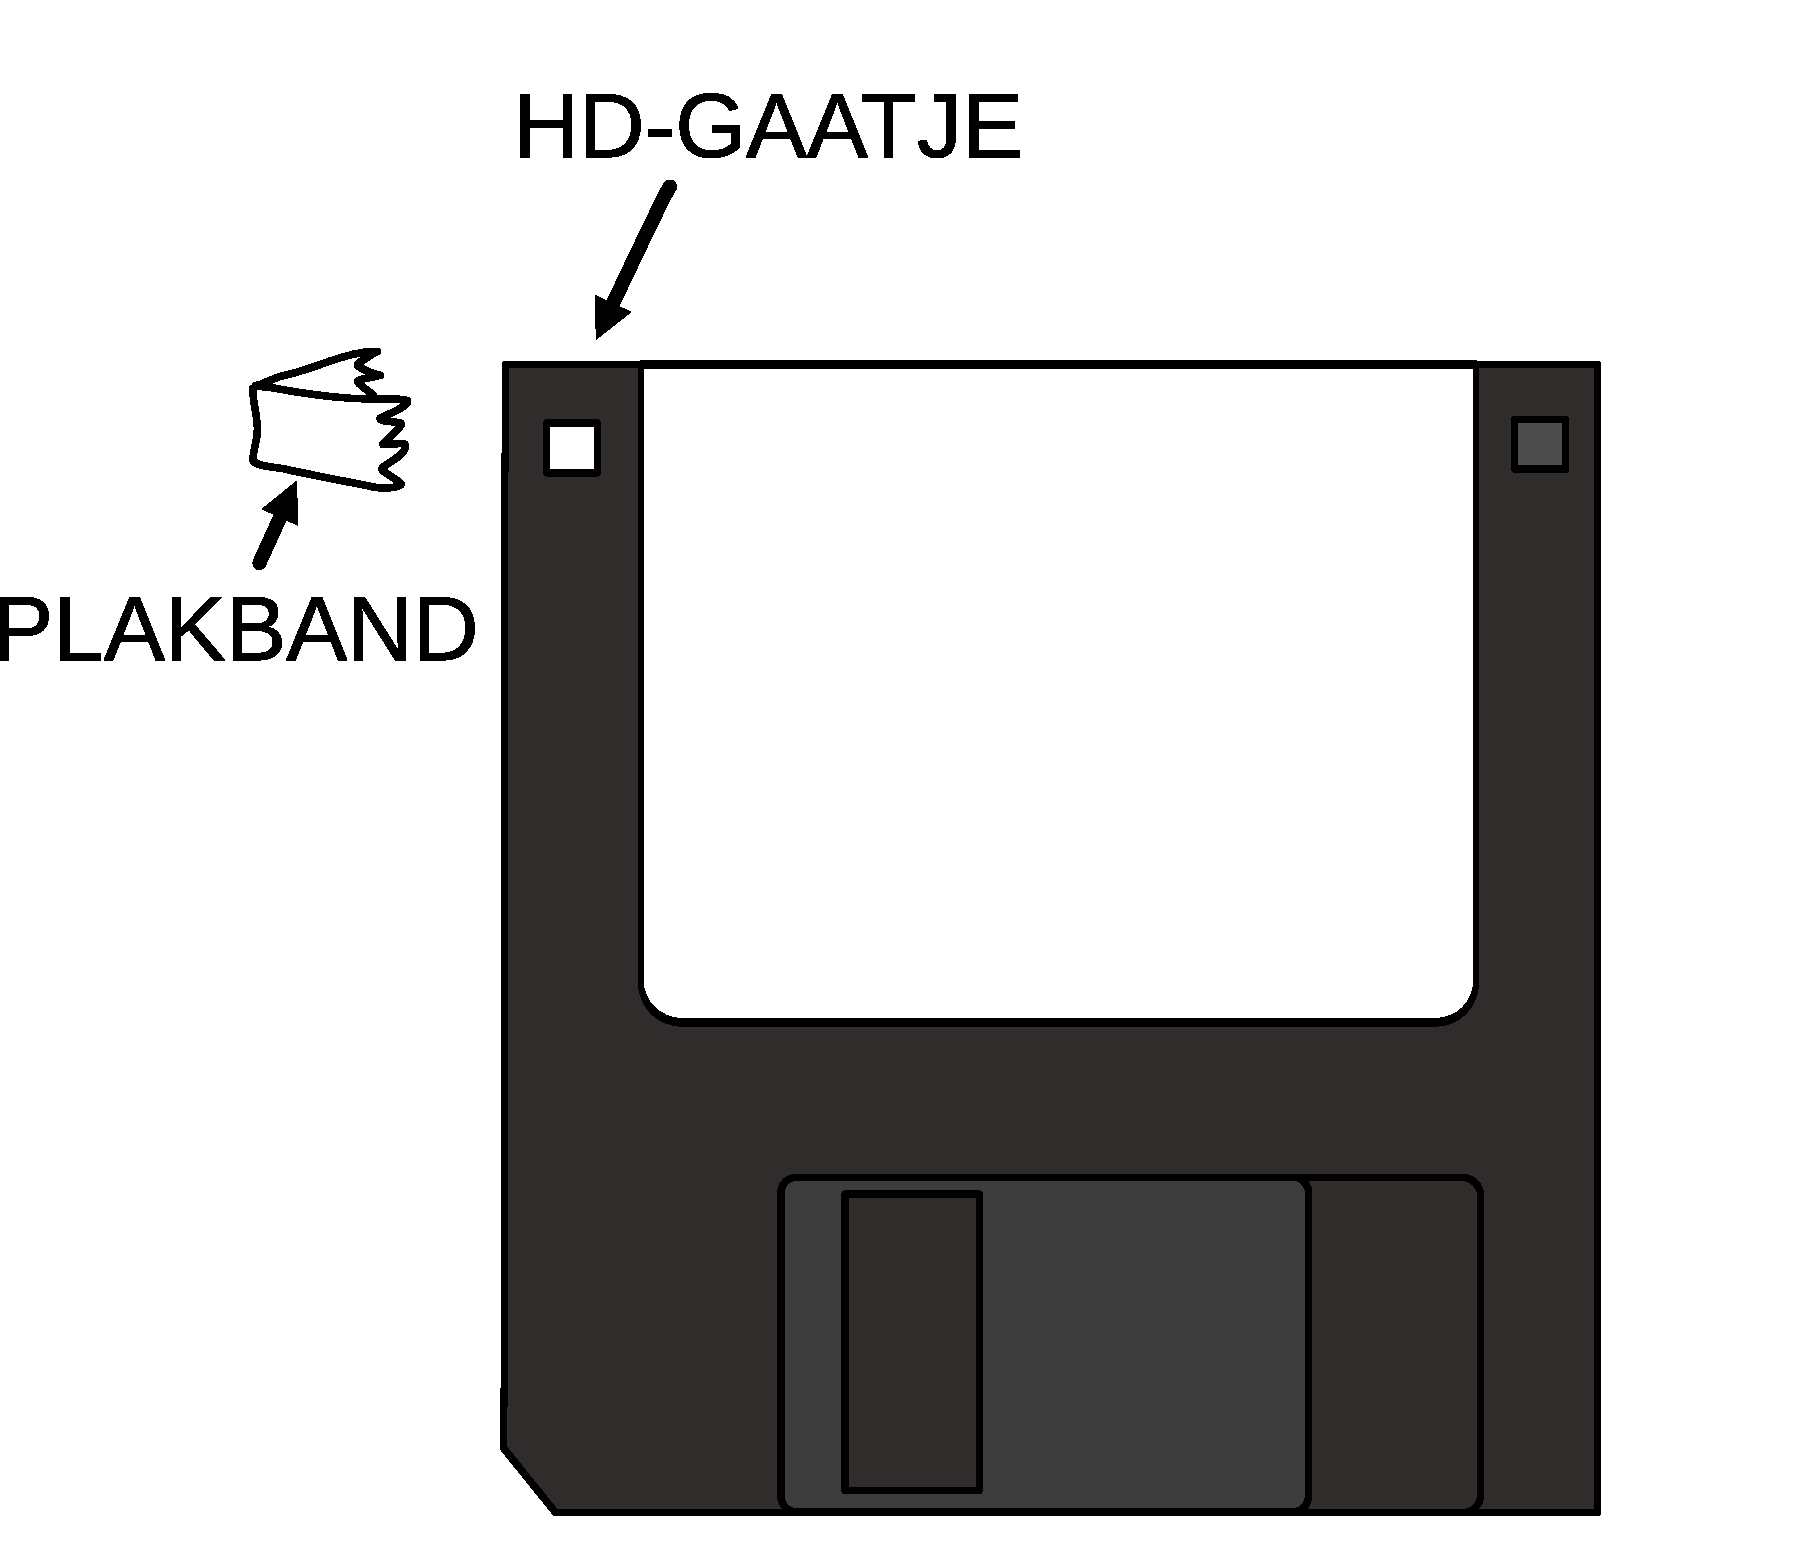
\includegraphics[width=0.75\textwidth]{dutch/images/illustrations/floppy_hd.pdf}
\end{center}

\underline{OPMERKING}: Zorg ervoor dat het plakband beide zijden van het gat bedekt.

\subsection{Een schijf formatteren}
\index{Schijfstations!Een schijf formatteren}

Een diskette moet geformatteerd worden voordat deze gebruikt kan worden. Het ingebouwde 3.5"-diskettestation van de MEGA65 emuleert een Commodore 1581-station en kan schijven gebruiken die in een dergelijk station zijn geformatteerd. U kunt een schijf ook met de MEGA65 formatteren.

\underline{OPMERKING}: Het formatteren van een schijf wist de inhoud ervan. Wees voorzichtig en doe dit uitsluitend wanneer u de gegevens op de schijf niet meer nodig hebt!

Voer de volgende stappen uit om een fysieke 3.5"-diskette met het interne station te formatteren:

\begin{enumerate}
\item Open het Freezer-menu.\index{Freezer-menu}\item Koppel het ingebouwde 3.5"-diskettestation aan het eerste beheerde station, unit 8.\item {\it Controleer dat unit 8 het volgende aangeeft:} \screentext{- INTERNAL 3.5" -}\item Hervat de computer: druk op \megakey{F3}.\item Plaats de diskette die u wilt formatteren in het interne diskettestation.\item Voer het BASIC-commando {\bf FORMAT} in en geef de schijf een naam ({\tt "MIJNDISK"}) en een ID van twee tekens ({\tt XX}).\index{BASIC 65-commando's!FORMAT}\index{BASIC 65-voorbeelden!FORMAT}
\begin{screencode}
FORMAT "MIJNDISK",IXX
\end{screencode}
\item Voer, wanneer u daarom gevraagd wordt, {\tt YES} in en druk op \widekey{RETURN}.
\end{enumerate}

Het formatteren van de schijf duurt ongeveer een minuut. Het station maakt tijdens het formatteren zoemende en klikkende geluiden. Schakel de computer niet uit en werp de schijf niet uit voordat het formatteren is voltooid.

U kunt bevestigen dat het formatteren is geslaagd door het {\bf DIR}-commando uit te voeren.\index{BASIC 65-commando's!DIR} U ziet dan een lege lijst van mappen met de naam en de ID die u hebt opgegeven. Uw schijf is nu gereed voor gebruik.


\section{Externe IEC-schijfstations gebruiken}
\index{Aansluitingen!IEC}

De MEGA65 werkt met externe schijfstations die op de seriële IEC-poort zijn aangesloten.

Externe stations hoeven niet te worden gekoppeld. Indien een unitnummer niet aan het ingebouwde 3.5"-diskettestation of aan een schijfimage is toegewezen, worden de schijfbewerkingen voor dat unitnummer naar de seriële IEC-poort verzonden. Het is aan het apparaat dat op de poort is aangesloten om zijn unitnummer te herkennen. Sommige IEC-apparaten hebben schakelaars waarmee u het unitnummer kunt instellen. Andere werken alleen met een specifiek nummer.

Indien u een extern station hebt dat een specifiek unitnummer verwacht, moet u ervoor zorgen dat de MEGA65 dat nummer niet aan een schijfimage of aan het interne station toewijst. Open het Freezer-menu\index{Freezer-menu} en druk vervolgens op \megakey{8} of \megakey{9} om de unitnummertoewijzingen om te schakelen, zodat zij het benodigde unitnummer niet meer gebruiken.\index{Unitnummer (IEC-apparaten)}

De station- en unitnummertoewijzingen zijn tijdelijk en worden teruggezet op hun standaardwaarden wanneer de MEGA65 wordt uitgeschakeld. U zult de stationtoewijzingen opnieuw moeten instellen wanneer u de computer de volgende keer inschakelt.


\section{Opstartbare schijven}
\index{Schijfstations!Opstartbare schijven}

Bij oudere Commodore-computers was het gebruikelijk dat softwaremakers de map op een diskette zo organiseerden dat het eerste bestand in de lijst het hoofdprogramma is. De gebruiker kon dan het commando \screentext{LOAD "*",8,1} invoeren om het hoofdprogramma te laden en \screentext{RUN} om het uit te voeren. Het sterretje is een jokerteken dat met elk bestand overeenkomt, dus ook met het eerste bestand op de schijf, zonder dat de gebruiker de naam van het programma hoeft te typen.

Deze methode is nog steeds gebruikelijk en de MEGA65 biedt een snelle manier om dergelijke schijven op te starten: houd \specialkey{SHIFT} ingedrukt en druk op \specialkey{RUN\\STOP}. Dit voert het commando \screentext{RUN "*"} uit, hetwelk vergelijkbaar is met de bekende commandoreeks die het eerste programma op de schijf laadt en uitvoert.\index{BASIC 65-commando's!RUN}

Met de C65 introduceerde Commodore een nieuwe manier om schijven op te starten. In plaats van te vertrouwen op de volgorde van bestanden, kan een schijf een bestand bevatten met de naam {\tt AUTOBOOT.C65}.\index{AUTOBOOT.C65-bestand} Indien dit bestand bestaat en een programma is, laadt en voert het BASIC-commando {\bf BOOT} dit bestand uit.\index{BASIC 65-commando's!BOOT}\index{BASIC 65-voorbeelden!BOOT}

\begin{screencode}
BOOT
\end{screencode}

\subsection{Schijven automatisch opstarten}

Zoals besproken in hoofdstuk \vref{cha:configuringyourmega}, kunt u het Configuratiehulpprogramma\index{Configuratie!Hulpprogramma} gebruiken om de MEGA65 in te stellen zodat hij tijdens het opstarten automatisch een virtueel schijfimage of het ingebouwde 3.5"-diskettestation koppelt.

Indien de gekoppelde schijf opstartbaar is --- dat wil zeggen dat hij een programmabestand met de naam {\tt AUTOBOOT.C65} bevat --- laadt en voert de MEGA65 het opstartprogramma automatisch uit.

Zo werkt de Intro Disk. Het Intro Disk-menu is een programma met de naam {\tt AUTOBOOT.C65} op het virtuele schijfimage {\tt MEGA65.D81}, hetwelk vooraf is ingesteld om bij het opstarten van het systeem gekoppeld te worden. Wanneer u de Intro Disk via het menu uitschakelt, hernoemt hij {\tt AUTOBOOT.C65} naar {\tt MENU}, zodat de schijf niet langer als opstartbaar wordt beschouwd.

Zelf een opstartschijf inrichten is een handige manier om uw computer te configureren. U kunt een kort BASIC-programma schrijven dat het systeemlettertype wijzigt, de achtergrondkleur aanpast en {\bf KEY}-macro's naar uw smaak instelt. Sla dit programma vervolgens op als {\tt AUTOBOOT.C65} op een schijf die u hebt geconfigureerd om bij het opstarten van het systeem aan te koppelen. Dit programma wordt elke keer uitgevoerd wanneer u uw MEGA65 inschakelt.


\section{De SD-kaart benaderen vanuit BASIC}

Verscheidene BASIC 65-commando's kunnen rechtstreeks op de SD-kaart van de MEGA65 werken alsof deze een schijfstation is. In deze gevallen staat de SD-kaart bekend als unit 12.

\underline{OPMERKING}: Unit 12 kan slechts voor enkele specifieke bewerkingen rechtstreeks worden benaderd. Hij kan de gehele SD-kaart niet als een CBDOS-schijf behandelen.

Om alle bestanden op de SD-kaart weer te geven, gebruikt u het {\bf DIR}-commando met het argument \screentext{U12}:\index{BASIC 65-commando's!DIR}\index{BASIC 65-voorbeelden!DIR}

\begin{screencode}
DIR U12
\end{screencode}

U kunt de optionele {\bf P}-vlag met dit commando gebruiken om de bestanden op de SD-kaart één pagina tegelijk weer te geven. Druk op Q om op de huidige pagina te stoppen, of op een willekeurige andere toets om naar de volgende pagina te gaan.

\begin{screencode}
DIR U12,P
\end{screencode}

Om een PRG-bestand rechtstreeks van de SD-kaart te laden (dat zich niet in een schijfimage bevindt), gebruikt u het \screentext{U12}-argument bij het {\bf DLOAD}-commando. In dit geval {\em moet} u het achtervoegsel {\tt .PRG} van de bestandsnaam opnemen, hetgeen verschilt van het gebruik van PRG-bestanden op schijven of in schijfimages. {\bf DSAVE} kan niet naar de SD-kaart opslaan met \screentext{U12} en meldt een fout als u het toch probeert; sla een programma daarom op in een schijfimage.\index{BASIC 65-commando's!DLOAD}\index{BASIC 65-commando's!DSAVE}\index{BASIC 65-voorbeelden!DLOAD}

\begin{screencode}
DLOAD "MIJNPROGJE.PRG",U12
\end{screencode}

Zoals eerder is besproken, ondersteunt de MEGA65 submappen op de SD-kaart en houdt een huidige werkmap bij voor schijfbewerkingen. Om de huidige werkmap te wijzigen naar een submap:\index{BASIC 65-commando's!CHDIR}\index{BASIC 65-voorbeelden!CHDIR}

\begin{screencode}
CHDIR "SUBDIR",U12
\end{screencode}

Om de huidige werkmap te wijzigen naar de bovenliggende map:

\begin{screencode}
CHDIR "..",U12
\end{screencode}

Het {\bf MOUNT}-commando kan een D81- of D64-schijfimage aan een unitnummer koppelen. Hoewel dit commando naar een bestand op de SD-kaart verwijst, maakt het geen gebruik van het \screentext{U12}-argument. In plaats daarvan stelt het commando met het {\bf U}-argument het unitnummer van de aan te koppelen schijf in. Het {\bf MOUNT}-commando gebruikt de door {\bf CHDIR} ingestelde huidige werkmap om het bestand te vinden.


\section{Gangbare schijfbewerkingen}

Hieronder vindt u enkele voorbeelden van gangbare schijfbewerkingen die u bij de \screentext{READY}-prompt kunt uitvoeren. Raadpleeg voor meer informatie de naslag over BASIC-commando's in bijlage \vref{cha:basic-reference}.

De meeste commando's die bestandsnamen aanvaarden, aanvaarden ook een {\bf U}-argument waarmee u aangeeft welke unit het bestand bevat. De standaardunit is 8.\footnote{Wanneer de computer voor het eerst wordt gestart, is de standaard schijfunit voor BASIC-commando's 8. U kunt deze wijzigen met het {\bf SET DEF}-commando.\index{BASIC 65-commando's!SET}}

\subsection{DIR}
\index{BASIC 65-commando's!DIR}\index{BASIC 65-voorbeelden!DIR}

Om de map (de lijst van bestanden) van een schijf weer te geven, gebruikt u het {\bf DIR}-commando.

\begin{screencode}
DIR

DIR U9
\end{screencode}

In tegenstelling tot de methode van de Commodore 64, waarbij de schijfmap in het BASIC-geheugen wordt geladen, wijzigt het {\bf DIR}-commando het BASIC-geheugen niet. U kunt {\bf DIR} veilig gebruiken wanneer er een programma in het geheugen staat.

Om grotere mappen gemakkelijker te kunnen bekijken, geeft {\bf DIR W} (van ``wide'') de map in kolommen weer en pauzeert na elke pagina.

\subsection{DLOAD en RUN}
\index{BASIC 65-commando's!DLOAD}\index{BASIC 65-voorbeelden!DLOAD}
\index{BASIC 65-commando's!RUN}\index{BASIC 65-voorbeelden!RUN}

Het {\bf DLOAD}-commando laadt een programma van de schijf in het geheugen. Het {\bf RUN}-commando voert het programma uit dat zich momenteel in het geheugen bevindt.

\begin{screencode}
DLOAD "GAAFSPEL"
RUN
\end{screencode}

U kunt beide tot één commando combineren door de bestandsnaam rechtstreeks aan het {\bf RUN}-commando te geven.

\begin{screencode}
RUN "GAAFSPEL"
\end{screencode}

\subsection{DSAVE}
\index{BASIC 65-commando's!DSAVE}\index{BASIC 65-voorbeelden!DSAVE}

Het {\bf DSAVE}-commando slaat het BASIC-programma dat zich momenteel in het geheugen bevindt op de schijf op.

\begin{screencode}
DSAVE "MIJNSPEL"
\end{screencode}

Standaard overschrijft dit geen bestaand bestand met dezelfde naam. Om een bestaand bestand te laten overschrijven, plaatst u een apestaartje vóór de bestandsnaam, binnen de dubbele aanhalingstekens.

\begin{screencode}
DSAVE "@MIJNSPEL"
\end{screencode}

Merk op dat opslaan met vervanging alleen wordt aanbevolen bij gebruik van schijfimages en het 3.5"-diskettestation. Oudere Commodore-stations bevatten fouten in deze functie die tot gegevensverlies kunnen leiden.

\subsection{BACKUP}
\index{BASIC 65-commando's!BACKUP}\index{BASIC 65-voorbeelden!BACKUP}

Het {\bf BACKUP}-commando kopieert een volledige schijf van de ene unit naar de andere. Hierbij worden alle bestaande gegevens op de bestemmingsschijf gewist.

\begin{screencode}
BACKUP U8 TO U9
\end{screencode}

U kunt {\bf BACKUP} gebruiken om schijfimages van floppy-schijven te maken, schijfimages naar floppy-schijven te schrijven of alles van het ene schijfstation naar het andere te kopiëren.

\subsection{COPY}
\index{BASIC 65-commando's!COPY}\index{BASIC 65-voorbeelden!COPY}

Het {\bf COPY}-commando maakt een kopie van een bestand. Indien bron en bestemming verschillende bestandsnamen op dezelfde unit zijn, dupliceert dit het bestand op de schijf. Wanneer u een bestand tussen units kopieert, behoudt het bestand zijn oorspronkelijke bestandsnaam. (Het nieuwe bestand kan met een afzonderlijk commando worden hernoemd.)

\begin{screencode}
COPY "MIJNSPEL", U8 TO U9

COPY "MIJNSPEL" TO "MIJNSPEL-V1"
\end{screencode}

\subsection{RENAME}
\index{BASIC 65-commando's!RENAME}\index{BASIC 65-voorbeelden!RENAME}

Het {\bf RENAME}-commando wijzigt de naam van een bestaand bestand.

\begin{screencode}
RENAME "MIJNSPEL-V29" TO "MIJNSPEL-GEREED"
\end{screencode}

\subsection{DELETE}
\index{BASIC 65-commando's!DELETE}\index{BASIC 65-voorbeelden!DELETE}

Het {\bf DELETE}-commando verwijdert een bestand.

\begin{screencode}
DELETE "ROMMELBESTAND"
\end{screencode}


\subsection{Snelkoppelingen voor schijfcommando's}

BASIC 65 biedt enkele snelkoppelingen voor gangbare schijfcommando's die u bij de \screentext{READY}-prompt kunt gebruiken.

\begin{center}
\begin{tabular}{|l|l|}
\hline
{\bf Snelkoppeling} & {\bf Overeenkomend commando} \\
\hline
\screentextwide{/} & {\bf LOAD} \\
\hline
$\uparrow$ & {\bf RUN} \\
\hline
$\leftarrow$ & {\bf SAVE} \\
\hline
\screentextwide{@} & {\bf DISK} \\
\hline
\screentextwide{\$} & {\bf DIR} \\
\hline
\end{tabular}
\end{center}

Deze snelkoppelingen zijn bedoeld om samen met een lijst van mappen programma's te starten zonder dat u bestandsnamen hoeft te typen. Bijvoorbeeld:

\begin{enumerate}
\item Geef de lijst van mappen van de schijf weer: typ {\bf \$} in en druk op \widekey{RETURN}.\item Gebruik de cursortoetsen om de cursor te verplaatsen naar de regel met het programma dat u wilt uitvoeren.\item Typ {\bf \screentext{$\uparrow$}} in en druk op \widekey{RETURN}.
\end{enumerate}

Het geselecteerde programma wordt geladen en uitgevoerd. Merk op dat u geen overtollige tekens van de regel hoeft te verwijderen. De snelkoppeling negeert alles behalve de bestandsnaam tussen dubbele aanhalingstekens, zoals die door de lijst van mappen wordt weergegeven.
